%!TEX root = main.tex

\section{Understanding Web Search Performance}
\label{sec:web_search}

\begin{table*}[th]
\caption{High-level statistics of web search flows.}
\label{tab:web_stats}
\centering
\renewcommand{\arraystretch}{1.0}
\begin{tabular}{c|c|c|c|C{1.2cm}|C{1.85cm}|C{2.1cm}}
	\hline
	& {finish time (sec.)} & {flow size (\#pkts)} & {RTT (ms)} & pkt loss rate & \% of flows w/ lost pkts & \% of flows w/ timeout retrx \\
	\hline
	WiFi & 0.197 (0.030, 4.608) & 9.0 (1.0, 33.0) & 39 (10, 372) & 3.0\% & 9.76\% & 4.1\% \\
	\hline
	3G & 0.124 (0.015, 0.440) & 19.0 (1.0, 82.0) & 38 (4, 68) & 0.9\% & 8.7\% & 0.1\% \\
	\hline
\end{tabular}
\end{table*}

We examine the TCP performance of web search flows in this section. We first provide a high-level statistics on the key performance factors in Table \ref{tab:web_stats}. For finish time, flow size and RTT, we report the median along with the $5th$ percentile and $95th$ percentile values in the parenthesis. The flow size measures the number of web search result packets as show in Figure \ref{fig:web_finish_time_example}. We observe a larger flow size of 3G flows than WiFi flows, which might be explained the difference in search behavior \cite{Song:2013:EEU:2488388.2488493}. Nevertheless, most of the flows contain no more than 100 packets for search results, implying that any TCP performance degradation (like a high packet loss) could exert a large impact on the user perceived latency (i.e. finish time) \cite{flach2013reducing}. The Kendall correlation coefficient between flow size and finish time is 0.018, indicating flow size has no impact on the finish time. Notably, 3G flows show smaller RTT, lower packet loss rate and also are less likely to suffer from the expensive timeout retransmissions. 
%\begin{figure}[th]
%\centering
%	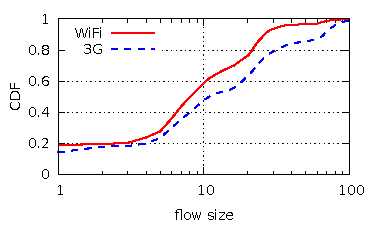
\includegraphics[width=0.8\linewidth]{web_flow_size}
%\caption{The distribution of flow sizes in web search.}
%\label{fig:web_flow_size}
%\end{figure}
%
%Figure~\ref{fig:web_flow_size} plots the distribution of flow size (measured by the number of web search result packets) in web search. The flow size varies from 1 packet to 100 packets with a median around 10 packets. Such a small flow size implies that any TCP performance degradation (like a high packet loss) could exert a large impact on the user perceived latency (i.e. finish time) \cite{flach2013reducing}. We also observe a smaller flow size of WiFi search than that of 3G search, which might be due to the difference in search behavior \cite{Song:2013:EEU:2488388.2488493}. We use Kendall correlation to determine whether flow size is relevant to finish time. The coefficient is 0.018, which demonstrates their irrelevance.

As a TCP sender in web search, the server can measure abundant TCP performance factors and behavior, enabling us to perform a detailed analysis of the TCP performance and its impact on the finish time. In what follows, we analyze the TCP performance in 3 main TCP stages and then particularly examine the timeout retransmissions.


\subsection{TCP Stage Analysis}

\begin{figure}[th]
\centering
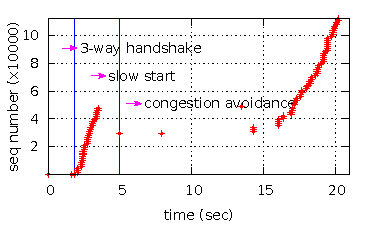
\includegraphics[width=0.8\linewidth]{web_three_stages}
\caption{The three stages in web search flows.}
\label{fig:web_three_stages}
\end{figure}

A TCP comprises 3 stages: \emph{3-way handshake}, \emph{slow start}, \emph{congestion avoidance}, which is exemplified in Figure~\ref{fig:web_three_stages} using a web search flow from our dataset, where $y$-axis shows the TCP sequence number. The TCP 3-way handshake (3WHS) stage ideally (i.e. without packet loss, delay and reordering) completes within 1 RTT. The server then enters the slow start stage, during which server does not encounter any packet loss or reordering event, and thus enlarges the congestion window by 1 segment size for each received ACK. The server enters congestion avoidance stage once it estimates a packet loss\footnote{The packet can actually be delayed or lost.}. In this stage, the server reduces the congestion window when detecting packet loss through fast retransmit\cite{rfc6675} and compels the congestion window to grow from 1 segment size when detecting packet loss through RTO. Note that the congestion avoidance stage here starts when server detects congestion event and ends till the flow finishes, which is slightly different from the TCP congestion avoidance stage in TCP/IP stack \cite{jacobson1988congestion}.

%Figure~\ref{fig:web_three_stages} gives an exemplified flow with 3 TCP stages that we define. The $y$-axis shows the TCP sequence number. In the figure, server takes 1.8s to establish connection, 3.1s to transmit 35 data packets in slow start stage, and 15.3s to transmit the left 48 data packets in congestion avoidance stage. In the following, we use the criteria of partitioning to break the analysis down into the three stages that flows experience.

\subsubsection{3-way Handshake}

\begin{figure}[th]
\centering
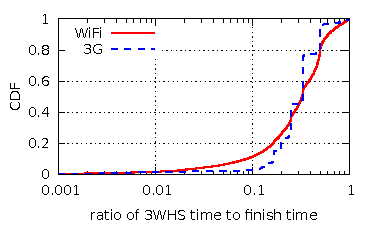
\includegraphics[width=0.8\linewidth]{web_handshake_time_ratio}
\caption{The ratio of time in 3-way handshake to finish time in each flow.}
\label{fig:web_handshake_ratio}
\end{figure}

We first examine how much of the time spent in the 3WSH stage in Figure~\ref{fig:web_handshake_ratio}, where we plot the ratio of the time in 3WSH to the finish time. Note that the $x$-axis is in log scale. 3G and WiFi flows spend similar ratio of time in this stage. We observe that the time for connection establishment can take up to half of the finish time for 30\% flows. More surprisingly, about 8\% of the WiFi flows and 3\% of 3G flows spend 70\% of their time during this stage. The small flow size is one of the reason for this observation. The maximum flow size is less than 100 packets as shown in Table~\ref{tab:web_stats}, implying the data can be transmitted within only a few RTTs if no congestion event happens. Such a short period of transmission time leads to a relatively large portion of time for connection establishment.


%From the figure, flows in cellular network have similar ratio of time in 3-way handshake to that in WiFi network (with median value 0.3). If the 3WSH could be removed from finish time, the user-perceived web search latency would be reduced by 30\% in more than half of the flows. Moreover, there are 8\% of flows in WiFi network consuming 70\% of their time in 3WSH.

%The unexpectedly high ratio of 3WSH could be introduced by two reasons. First, most of web search flows contains packets ranging from 1 to 100, these data could transmitted in 1 to 4 RTT's if there is no congestion event. Thus 3WHS, without transmitting any data, occupies a large fraction of time in short flows. Second, there are a non-negligible fraction of flows experiencing SYN retransmission during 3WHS stage. 

Another important reason that explains the unexpectedly long time in 3WSH stage (i.e. $>70\%$ of finish time) is the timeout retransmissions in this stage. As the data packets cannot be transmitted before a TCP connection is established, a loss of SYN will lead to a timeout retransmission, which takes 1 second (\ie the initial RTO) to retransmit the SYN. We find that 4.4\% of WiFi search flows and 0.5\% of 3G flows experience at least one SYN timeout retransmission. A timeout retransmission of SYN also reduces the congestion window size to 1, further hurt the data transmission performance. We envision a possible way to mitigate the costly 3WSH in such short flows where clients maintain long-term TCP connections to the web search servers.

\subsubsection{Slow Start Stage}

\begin{figure}[th]
\centering
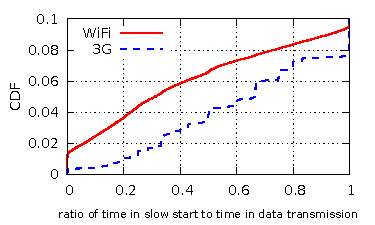
\includegraphics[width=0.8\linewidth]{web_slowstart_time_ratio}
\caption{The ratio of time in slow start to the time in data transmission.}
\label{fig:web_ss_time_ratio}
\end{figure}

The slow start stage and the congestion avoidance stage constitute the data transmission period. Figure~\ref{fig:web_ss_time_ratio} shows the ratio of time in slow start stage to the time spent in data transmission (\ie the sum of time in slow start and congestion avoidance stages). Note that the $y$-axis is capped at 0.1. It can be seen that 1.5\% of the WiFi flows is unable to transmit any data in the slow start stage, because the first packet is dropped. We indeed find of the flows that experience the congestion avoidance stage, the packet loss happens within the first congestion window (i.e. within the first 10 packets) for 80\% of WiFi flows.

\begin{table}[th]
\caption{Comparison of finish time (second) for flows finishing in the slow start stage and those not.}
\label{tab:web_finish_time_3rd_stage}
\centering
\renewcommand{\arraystretch}{1.0}

\begin{tabular}{l|c|c|c}
\hline
& 5 \%ile & median & 95 \%ile \\
\hline
WiFi finished & 0.03 & 0.17 & 2.81 \\
WiFi unfinished & 0.08 & 0.77 & 21.24 \\
%\hline

\hline
3G finished & 0.01 & 0.12 & 0.81 \\
3G unfinished & 0.01 & 0.16 & 2.42 \\
%\hline

\hline
\end{tabular}
\end{table}

More importantly, regardless of the access type, more than 90\% of the flows finish in the slow start stage. In other words, about 10\% of the flows have to experience the congestion avoidance stage. Intuitively, a longer time in slow start stage, the shorter time to complete the data transmission. To examine this, we compare the finish time in Table \ref{tab:web_finish_time_3rd_stage} between flows that finish in the slow start stage and those not. WiFi flows are more likely to be impacted by whether or not finishing in this stage. In other words, increasing the possibility of finishing web search results transferring in this stage can greatly improve the user perceived latency. For example, the median finish time would be improved by 4 times if a flow that enters the congestion avoidance stage finished in the slow start stage. The 95th percentile finish time even can be improved by one order of magnitude. 



%Another interesting observation is that 1.5\% of the WiFi flows is unable to transmit any data in the slow start stage as the first packet is dropped. We indeed find of the flows that experience the congestion avoidance stage, the packet loss happens within the first congestion window (i.e. within the first 10 packets) for 80\% of WiFi flows, while this percentage is only 20\% for 3G flows, implying a reconsideration of the initial congestion window configuration.

\begin{table}[th]
\caption{The correlation between RTT and finish time.}
\label{tab:web_rtt_finish_time_correlation}
\centering
\renewcommand{\arraystretch}{1.0}
\begin{tabular}{c|C{2.5cm}|C{2.5cm}}
   \hline
   & w/o 3rd stage & w/ 3rd stage \\
   \hline
   WiFi & 0.55 & 0.13 \\
 %  \hline
   3G & 0.59 & 0.52 \\
   \hline
\end{tabular}
\end{table}

During the slow start stage, the congestion window is doubled after each RTT. As such, RTT would have a high impact on the flow finish time. To examine this, we examine the Kendall correlation between RTT and finish time for flows that finish in the slow start stage (i.e. without entering the 3rd stage) in Table \ref{tab:web_rtt_finish_time_correlation}. For comparison, we also report the correlation for flows that experience the 3rd stage (i.e. congestion avoidance stage). We observe that regardless of the access type, a moderately high correlation for flows that finish in the slow start stage, confirming the relatively high impact of RTT on the finish time for these flows. The correlation for flows that experience the 3rd stage however is dependent on the access type, which can be explained by the fact that other factors, like packet loss, can have a significantly impact during the congestion avoidance stage. As we have seen in Table \ref{tab:web_stats}, WiFi flows experience a higher packet loss rate and thus are more likely to be impacted by the packet loss, rather than RTT. In addition, as we will see in the following analysis that WiFi flows that experience the 3rd stage are more likely to recover packet losses through expensive timeout retransmission. 


\subsubsection{Congestion Avoidance Stage}

\begin{figure}[th]
\centering
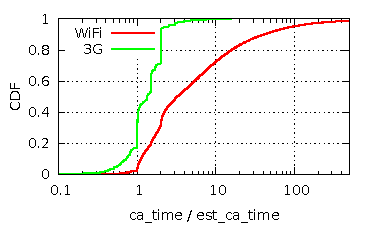
\includegraphics[width=0.8\linewidth]{web_ca_prac_over_est}
\caption{CDF of the extra time introduced by the congestion avoidance stage.}
\label{fig:web_ca_round}
\end{figure}

We first examine how much extra time the congestion avoidance stage introduces for individual flows. Let $\#(ca\_pkts)$ be the number of packets transmitted in this stage for a flow. As a TCP sender, the server sends $cwnd$ packets in one RTT, where $cwnd$ is the size of the congestion widow at the time when entering the congestion avoidance stage. Thus, if the flow had not experience the congestion avoidance stage, the server would have sent $\#(ca\_pkts)$ packets in a time frame of $T_e =  \left \lceil{\frac{\#(ca\_pkts)}{cwnd}} \right \rceil  \times RTT$. Now, we observe the flow actually spent $T_r$ of time for transmitting these packets. Then we compute the ratio of  $T_r$ to $T_e$ and use this ratio to measure the extra time introduced by the this stage. Unfortunately, we are unable to obtain $cwnd$ from the traces and thus alternatively use the number of in-flight packets at the time when entering the stage to approximate this value\cite{rfc56812009tcp}. 


 
Figure \ref{fig:web_ca_round} reports the distribution of this ratio. We observe a surprisingly high ratio for WiFi flows. The median ratio is as high as 3.2 and 20\% of the WiFi flows has a ratio more than 11, meaning a 10 times extra time is introduced for these 20\% of flows. 3G flows on the other hand have a ratio no more than 2 for 95\% of the flows. The difference of 3G and WiFi flows in the packet loss rate (3\% in WiFi versus 0.9\% in 3G) and the difference in the impact of packet loss should contribute most to the huge difference between WiFi and 3G flows observed. 



\begin{table}[th]
\caption{The finish time (in second, represented as $mean$ ($5th$ percentile, $95th$ percentile)) under different number of lost packets.}
\label{tab:web_loss_finish_time}
\centering
\renewcommand{\arraystretch}{1.0}
\begin{tabular}{c|c|c}
\hline
\#(lost pkts) & WiFi & 3G\\
\hline
0 & 0.18 (0.03, 3.20) & 0.12 (0.01, 0.57) \\
%
1 & 0.48 (0.05, 12.07) & 0.22 (0.04, 0.57) \\
%
2 & 0.54 (0.08, 14.46) & 0.23 (0.04, 0.59) \\
%
$\ge$3 & 2.82 (0.14, 34.89) & 0.27 (0.05, 0.93) \\
\hline
\end{tabular}
\end{table}


We then examine the impact of packet loss on finish time in Table \ref{tab:web_loss_finish_time}. Flows are grouped based on how many packets were lost in individual flows. The median of the finish time, along with the $5th$ percentile and $95th$ percentile values of each group are reported. For comparison, we also report the statistics for flows without any packet loss (i.e. these flows finish the data transmission in the slow start stage). For 3G flows, a packet loss increases the flow finish time by about one fold compared to the flows with no packet loss. A higher number of packet loss more than 1 does not increase the finish time significantly. Moreover, it seems that packet loss has a higher impact on finish time for WiFi flows than 3G flows. For example, the median finish time increases from 180 ms for flows with no packet loss to 480 ms for flows with 1 lost packets, and grows up to 2.8 second for flows with more than 3 lost packets. 

The huge difference in the impact of packet loss on finish time for WiFi and 3G flows is related to how the packet loss is recovered. A packet loss can be recovered by either fast retransmit, limited retransmit~\cite{allman2001enhancing}, early retransmit~\cite{rfc5827}, or timeout retransmission by the server\footnote{TLP \cite{flach2013reducing} is not enabled in the server.}. Among these possible recovery methods, the most expensive one is the timeout retransmission, which is indeed the factor that explains the difference for WiFi and 3G flows observed in Table \ref{tab:web_loss_finish_time} as our following analysis reveals. 

\subsection{Timeout Retransmission Analysis}

\begin{figure}[th]
\centering
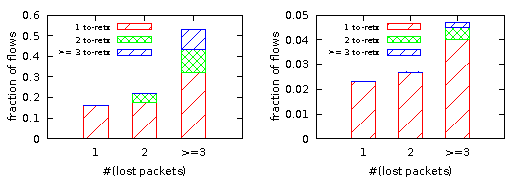
\includegraphics[width=\linewidth]{web_loss_rto_ratio}
\caption{The fraction of flows with timeout retransmission under different number of lost packets.}
\label{fig:web_loss_rto_ratio}
\end{figure}

%For each data packet which is not retransmitted, the measured RTT is the duration from that server transmits the packet, to that server receives the acknowledgment for it. In web search progress, we record as many RTT's as possible. When each new RTT is measured, the RTO value is updated by $RTO = SRTT + max(200ms, 4 RTTVAR)$, where $SRTT$ and $RTTVAR$ mean smoothed RTT and RTT variation respectively. For a retransmitted packet, if the duration between its retransmission time and the time that last packet is transmitted is larger than the calculated RTO, we could infer that it is a timeout retransmission. For each retransmitted packet, if server would not receive D-SACK, such a retransmission recovers a real packet loss, otherwise, the packet is not dropped and the retransmission is spurious. Note that a data segment could be retransmitted twice or more if the previously retransmitted packet is regarded as lost.





A retransmission is identified as a timeout retransmission if this retransmission happens at least a time frame of RTO after the transmission of the previous packet. The RTO here is computed as \cite{rfc62982011computing} $$RTO=\text{SRTT} + max(200ms, 4 \text{ RTTVAR})$$, where SRTT is the smoothed value of all measured RTTs, and RTTVAR is the variation of RTTs. We examine the fraction of flows that experience timeout retransmission(s) given the number of lost packets in Figure ~\ref{fig:web_loss_rto_ratio}. Note that the two sub-figures have different $y$-axis limitations. We can see that WiFi flows are more likely to suffer from timeout retransmissions than 3G flows. Given the same number of lost packets, the fraction of WiFi flows suffering from timeout retransmissions is about one order of magnitude higher than that of 3G flows. Another notable observation is that 20\% of WiFi flows having more than 3 packets lost experience more than 2 timeout retransmissions, which could lead to a serious performance degradation for these flows. This percentage however is only 1\% for 3G flows. 

An interesting question is then \textit{``why timeout retransmissions are more likely to happen for WiFi flows than 3G flows?''}. To answer this question, we need to nail down the reasons behind each timeout retransmission. Essentially, there are two scenarios in which a TCP sender has to appeal timeout retransmission for loss recovery. The first scenario is that the retransmitted packet issued, for example by fast retransmit, to recover the loss is dropped by network. In this case, the sender has to wait for a time frame of RTO to recover the packet loss (referred as \emph{double retransmission}). 

The second scenario is that the sender cannot collect sufficient number of duplicate acknowledgments (\emph{dupacks}) to trigger fast retransmit. The insufficiency of dupacks could be caused by various reasons: (1) the packet loss happens in the last 3 packets of a flow, referred as \emph{tail retransmission}~\cite{flach2013reducing}; (2) the congestion window is small (\eg 1 segment size after timeout retransmission), referred as \emph{small cwnd retransmission}; (3) the lost packet is followed subsequently by other packets with higher sequence numbers and the ACKs of subsequence packets are delayed for a long time (say longer than RTO), referred as \emph{packet delay retransmission}. The last case might be caused by large network latency jitters or by the middleboxes' behavior of blocking the dupacks~\cite{honda2011isit}. 

\begin{algorithm}
	\caption{Process of determining the type of timeout retransmission.}
	\label{alg:rto}
	\begin{algorithmic}[1]
		\Procedure{ParseRTO}{$timeout\ retx$}
			\If {packet has been retransmitted}
				\State \textbf{return} $double\_retransmission$
			\ElsIf {position to tail $\le$ 3}
				\State \textbf{return} $tail\_retransmission$
			\ElsIf {\#(in-flight packets) = 1}
				\State \textbf{return} $small\_cwnd\_retransmission$
			\ElsIf {only 1 in-flight packet is dropped \textbf{and}
				\Statex \indent\indent\indent\indent no dupack is received}
				\State \textbf{return} $packet\_delay\_retransmission$
			\Else
				\State \textbf{return} $others$
			\EndIf
		\EndProcedure
	\end{algorithmic}
\end{algorithm}

We use the method shown in Algorithm~\ref{alg:rto} to determine the type of timeout retransmission. Those that cannot be classified into any of the above type (e.g. when all packets in the windows are dropped) are labeled as others. Table \ref{tab:rto_type} reports the fraction of timeout retransmissions classified into each type.

\begin{table}[th]
\caption{Types of timeout retransmissions.}
\label{tab:rto_type}
\centering
\renewcommand{\arraystretch}{1.0}
\begin{tabular}{c|C{1.1cm}|C{1.1cm}}
	\hline
	{timeout retx type} & WiFi & 3G \\
	\hline
	tail retx & 38.3\% & 69.6\% \\
	double retx & 33.8\% & 13.5\% \\
	packet delay retx & 27.4\% & 16.1\% \\
	small cwnd retx & 0.3\% & 0.6\% \\
	others & 0.2\% & 0.2\%\\
	\hline
\end{tabular}
\end{table}

Tail retransmission contributes the majority (i.e. 70\%) of timeout retransmissions for 3G flows. Indeed, if the packet loss happens in the tail of a flow, it has to be recovered through timeout retransmission. Given the small size of web search flows, the tail packet loss can lead to a notable increase of finish time~\cite{flach2013reducing}. However in WiFi flows, only 38\% of the timeout retransmissions are classified as tail retransmissions, because double retransmission and packet delay retransmission become much more important than in the 3G flows. The higher probability of double retransmission in WiFi flows might come from the higher packet loss rate, in which case the retransmitted packet itself is dropped. On the other hand, the higher probability of packet delay retransmission implies a possibility that in WiFi network that we examined, middleboxes might buffer the disordered packets. We leave the examination of middleboxes effect as our future work.

The results in Table \ref{tab:rto_type} explain why timeout retransmissions are more likely to happen in WiFi flows: besides tail retransmissions, the loss of the retransmitted packet and the delayed ACKs also increase the likelihood of timeout retransmission greatly for WiFi flows, but they contribute much less in 3G flows. Our observations also implies that besides the mitigation method (like TLP \cite{flach2013reducing}) for tail retransmission, we also need methods to mitigate the double retransmissions and packet delay retransmissions, especially in WiFi network.

\subsection{Summary of web search analysis}

The key observations on web search flows are summarized below.

\begin{itemize}
	\item More than 50\% of flows spend at least 30\% of their total time on establishing connections. Moreover, 4.4\% of WiFi flows have to retransmit the SYN packet, making the time for establishing connections longer than 1 second.
	\item In 90\% of flows, RTT plays an important role in the finish time, due to no packe loss. However, in the flows with packet loss, the time spent on loss recovery dominates the finish time.
	\item When there are packet loss, the time for loss recovery make the finish time a t least 2-3 times larger. Compared with 3G flows, WiFi flows are more sensitive to packet loss. Under the same number of lost packets, WiFi flows experience much longer finish time than 3G flows.
	\item Most of timeout retransmissions in 3G network are induced by packet loss at flow tail. However, tail retransmission, double retransmission and packet delay retransmission occupy 38.3\%, 33.8\% and 27.4\% of timeout retransmissions in WiFi flows respectively. This is induced by both higher packet loss rate and misbehaving middleboxes.
\end{itemize}
